% ----------------------------------------------------------
% Glossário
% ----------------------------------------------------------
%
% Consulte o manual da classe abntex2 para orientações sobre o glossário.
%
%\glossary

% ----------------------------------------------------------
% Apêndices
% ----------------------------------------------------------

% ---
% Inicia os apêndices
% ---
\begin{apendicesenv}

% Imprime uma página indicando o início dos apêndices
\partapendices

% ----------------------------------------------------------
\chapter{\label{appendix:LC}Path length and clustering for regular ring lattices}
% ----------------------------------------------------------

\section{Average Path Length}

The distance $L_{ij}$ between two nodes $i$ and $j$ is the minimum number of edges that must be traversed to connect them. The average
path length is defined as the average distance between every possible pair of nodes in the network. For a network with $N$ nodes this
is:

\begin{equation}
    L = \frac{2}{N^2-N}\sum_{i<j}L_{ij}
\end{equation}

Consider the lowest node in a ring graph with $N$ nodes and $2K$ neighbors per node. Going counterclockwise (CCW), there are $K$ nodes
at distance $1$, then $K$ nodes at distance $2$ and so on until we reach some region near the top. In total, there will be $G$ groups
of nodes, each with $K$ nodes, at distances $1,2,3...,G$ from our starting point at the bottom. $G$ is given by the largest integer
smaller than $(N-1)/(2K)$. This can be written with the floor operation:

\begin{equation}
    G=\floor*{\frac{N-1}{2K}}
\end{equation}

This same procedure can be performed from the clockwise (CW) direction. Thus, there are $2K$ nodes at distance $1$ and so on up to
distance $G$. The last group of nodes at the top is therefore at a distance $G+1$, but it contains less than $2K$ nodes. Indeed, it
contains a number $R$ of nodes equal to the remainder of the integer division of $N-1$ by $2K$:

\begin{equation}
    R = N - 1 - 2KG
    \label{eq:R}
\end{equation}

\noindent This reasoning can be visualized in Fig.~\ref{fig:Lgroups}.

\begin{figure}
\centering
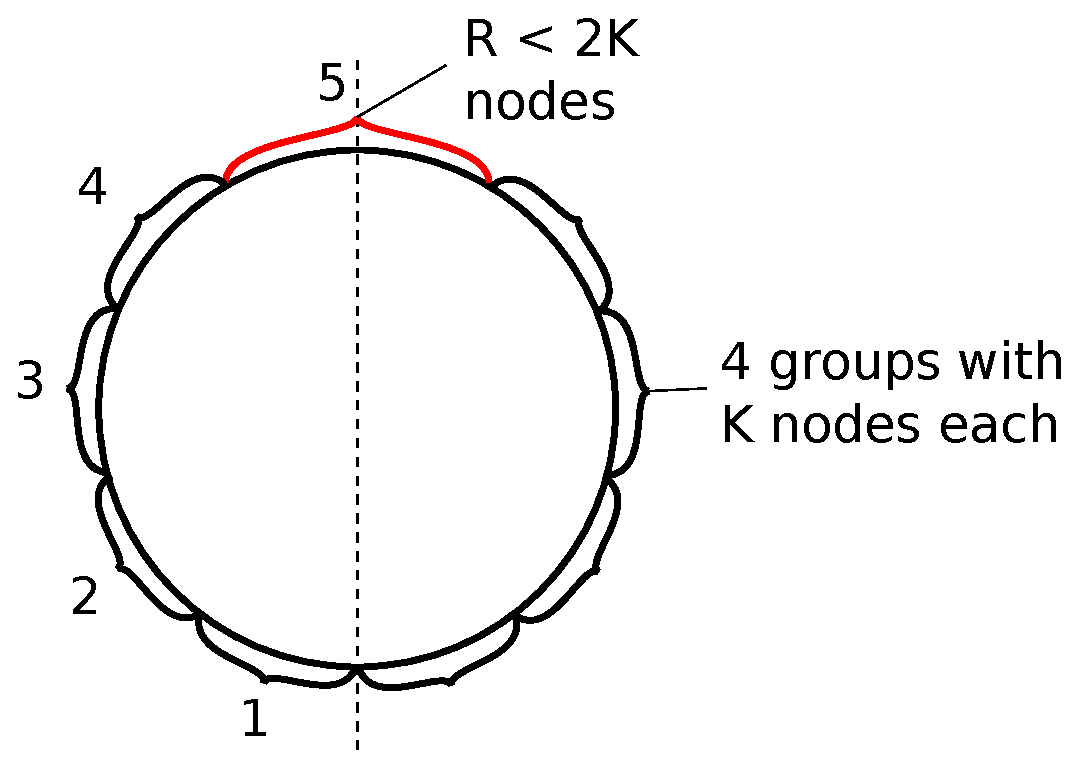
\includegraphics[width=0.6\textwidth]{fig/path_length_groups.eps}
\caption{Counting the number of nodes at distances visually. Here $G=4$ groups at distances $1,2,3,4$ from the bottom node.}
\label{fig:Lgroups}
\end{figure}

Since there are $N-1$ pairs between the bottom node and all other nodes in the lattice, the average distance $L_0$ between the bottom
node and all other nodes is then given by:

\begin{align}
    L_0 &= \frac{1}{N-1} \left[ 2K \sum_{i=1}^Gi + R(G+1) \right] \notag \\[9pt]
        &= \frac{1}{N-1} \left[ KG(G+1) + R(G+1) \right] \notag \\[9pt]
    L_0 &= \left(G + 1\right) \left( 1 - \frac{KG}{N-1} \right)
\end{align}

\noindent where we used equation \ref{eq:R} to substitute in for $R$.  Because we started with an arbitrary node at the bottom, this
result is true for any given node in a regular ring, and thus we conclude that the average path length for the whole network is just
$L_0$.

\begin{align}
    L(N,K) = \left(G + 1\right) \left( 1 - \frac{KG}{N-1} \right) \notag \\[9pt]
    \text{with} \qquad G=\floor*{\frac{N-1}{2K}}
\end{align}

\section{Average Clustering}

The clustering coefficient for a node $i$ in the graph is defined as: let $n_i$ be the number of neighbors of some node $i$. Then,
there are at most $(n_i^2-n_i)/2$ connections between any two of its neighbors. Let $m_i$ be the number of actual connections that are
present in a particular graph. Then, the clustering coefficient $C_i$ of node $i$ is given by:

\begin{equation}
    C_i = \frac{2m_i}{n_i^2-n_i}
\end{equation}

\noindent If there are $N$ nodes in the graph, the average clustering
coefficient is thus given by:

\begin{equation}
    C = \frac{1}{N}\sum^N_{i=1} C_i
\end{equation}

First, consider a ``close-up" of a section of a regular ring where $N\gg K$.  Consider a node $i$ with $K$ CW neighbors and $K$ CCW
neighbors. Let $m$ be the number of connections between neighbors of node $i$. We can manually count $m$ for some values of $K$:

\begin{figure}
\centering
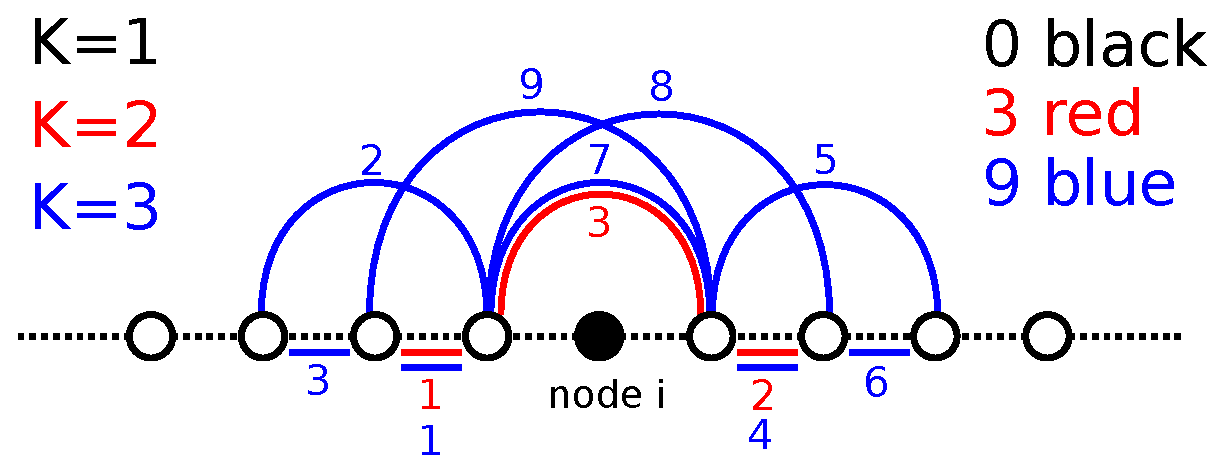
\includegraphics[width=0.75\textwidth]{fig/clustering.eps}
\caption{ (Color online) Counting $m$ for $k=1,2,3$. We note three contributions to $m$: a fully connected group of $K$ CW neighbors
(left), a fully connected group of $K$ CCW neighbors (right) and connections that go ``over" the center node.  }
\label{fig:clustering}
\end{figure}

\begin{align*}
    m &= 0 \qquad \text{if} \qquad K \leq 1\\
    m &= 3 \qquad \text{if} \qquad K = 2\\
    m &= 9 \qquad \text{if} \qquad K = 3
\end{align*}

The general case for $N \gg K$ can be counted by summing the contributions of the three groups as shown in figure \ref{fig:clustering}.
Two fully connected groups of $K$ nodes each contributes with $(K^2-K)$ connections. The connections that bypass node $i$ also
contribute with $(K^2-K)/2$ connections and thus we have.

\begin{align}
    m &= \frac{3}{2}(K^2-K)
    \label{eq:m}
\end{align}

\noindent Now we divide equation \ref{eq:m} by the total number of connections between the $2K$ neighbors of node $i$ to get its
clustering coefficient $C_i$:

\begin{align}
    C_i(N,K) = \frac{3K-3}{4K-2}
    \label{eq:ci}
\end{align}


\begin{figure}
\centering
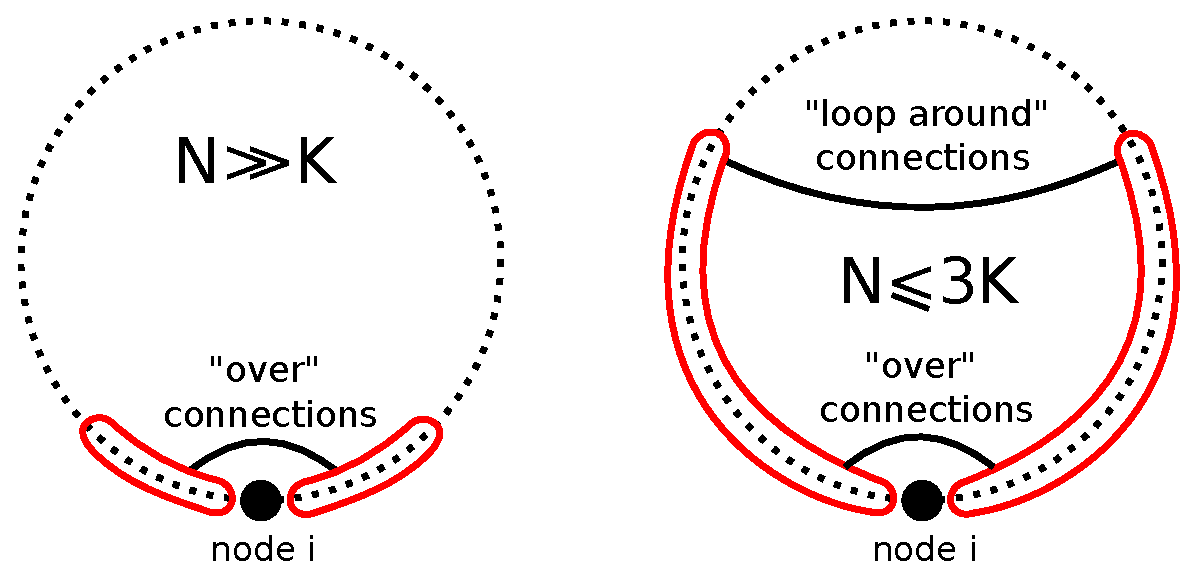
\includegraphics[width=0.9\textwidth]{fig/clustering-loop.eps}
\caption{ Connections that contribute to the clustering coefficient of node $i$.  The red regions represent the CW and CCW groups of
neighbors of node $i$, and they are fully connected each within itself. Additional connections are made going ``over" node $i$, but
when $N\leq3K$ there are additional connections that loop around the opposite side of the lattice.  }
\label{fig:loop}
\end{figure}

\noindent When $N$ is not so large compared to $K$, additional connections between the CCW and CW neighbors may appear by looping
around the opposite side of node $i$, as depicted in figure \ref{fig:loop}. These additional connections will be present whenever the
remaining nodes that are neither in the CW or CCW group are fewer than $K$. The number of such nodes is just $N-2K-1$, which gives us
the condition $N\leq 3K$ for additional connections to be present.


The number of ``loop around" connections that will be present will depend on how many nodes there are in the remaining group after
removing node $i$ and its immediate neighbors. Let this number be denoted by $D=N-2K-1$. Then, the number of additional connections
will be given by

\begin{align}
    (K-D) + (K-D-1) + ... + 2 + 1 = \frac{(K-D+1)(K-D)}{2}
    \label{eq:looparound}
\end{align}

Adding equation \ref{eq:looparound} to \ref{eq:m} we get

\begin{align}
    m = \frac{3}{2}(K^2 - K) + \frac{1}{2}(3K-N+1)(3K-N+2)
\end{align}

And thus the clustering now becomes:

\begin{align}
    C_i(N,K) = \frac{3K-3}{4K-2} + \frac{(3K-N+1)(3K-N+2)}{4K^2-2K}
    \label{eq:ci1}
\end{align}

This formula holds up to the point when $D=0$ or $N=2K+1$. For all values $D\leq 0$ the regular ring is in fact a complete graph, where
every node connects to every other. In these cases the clustering coefficient is always equal to one.  Formulas \ref{eq:ci} and
\ref{eq:ci1} together offer a complete expression for the clustering of node $i$. Since $C_i=C_j \quad \forall i,j$, this is just the
average clustering of the whole network and we finally get:

\begin{align}
    C(N,K) =
    \begin{cases}
        \frac{3K-3}{4K-2} \quad &\text{if} \quad N>3K \\[9pt]
        \frac{3K-3}{4K-2} + \frac{(3K-N+1)(3K-N+2)}{4K^2-2K} \quad &\text{if}
        \quad 3K \geq N > 2K+1 \\[9pt]
        1 \quad &\text{else}
    \end{cases}
    \label{eq:ci2}
\end{align}


\end{apendicesenv}


% ----------------------------------------------------------
% Annex
% ----------------------------------------------------------
%\begin{anexosenv}
%
%
%\partanexos  % Print annex front page
%
%\chapter{My annex 1}
%\chapter{My annex 2}
%
%
%\end{anexosenv}

%---------------------------------------------------------------------
% INDICE REMISSIVO - ELEMENTO OPCIONAL
%---------------------------------------------------------------------
%\phantompart
%\printindex
%---------------------------------------------------------------------
